\chapter{Introdução}
O coeficiente de absorção sonora de um material é um parâmetro muito utilizado para a caracterização de materiais acústicos. Através dele é possível determinar o impacto de uma amostra em um ambiente reverberante.

Esse trabalho teve como objetivo analisar o coeficiente de absorção sonora de uma amostra de um material poroso através de um tubo de impedância, ou seja, considerando apenas incidência direta de ondas sonoras sobre a amostra. Para isso, utilizou-se como base a norma ISO 10534-2:1998, que estabelece os procedimentos que devem ser feitos para determinar tal parâmetro.

O tubo de impedância deve ser construído de paredes rígidas e pode ter secção transversal circular ou quadrada, o que pode ser conveniente dependendo do tipo de amostra a ser caracterizada. No entanto, tubos de secção circular são mais usualmente utilizados devido a maior rigidez mecânica desta geometria, já que a norma especifica que as paredes do tubo devem ser rígidas de forma que modos de vibração na faixa de frequências de operação do tubo não sejam excitados por fontes externas ou pelo alto-falante. O tubo também deve ser reto e com secção interna constante (variabilidade < 0.2\%). 

As principais limitações associadas a este ensaio são que somente o coeficiente de absorção por incidência normal pode ser medido, já que o tubo de impedância assume ondas planas, e também uma limitação de faixa de frequências associada principalmente às dimensões da secção transversal do tubo. É muitas vezes necessário portanto construir um par de tubos de impedância e usar um deles para uma faixa de baixas frequências e outro para uma faixa de altas frequências. Tipicamente um bom aparato experimental pode medir o coeficiente de absorção em uma faixa entre 50 - 6000 [Hz]. Cuidados também devem ser tomados na inserção da amostra no tubo e no procedimento experimental.


\chapter{Formulação Analítica}

Em um duto pode-se considerar que há propagação de ondas planas até uma frequência superior, denominada frequência de corte. A partir dessa frequência, modos transversais de propagação começam a surgir, de modo que há não ocorrer somente propagações de ondas planas no duto. Para dutos de secção circular essa frequência superior pode ser definida através da Equação \ref{eq:frequencia_corte}.
\begin{equation}
f_{\text{corte}}=\frac{1,84c_{o}}{\pi d}\;,
\label{eq:frequencia_corte}
\end{equation}
\noindent{onde $c_{o}$ é a velocidade de propagação da onda sonora no ar e $d$ é o diâmetro do duto.}

Para frequências inferiores a frequência de corte a pressão sonora é dividida em duas partes, pressão sonora incidente e pressão sonora refletida. A pressão sonora de uma onda incidente $p_{i}$ e a pressão sonora de uma onda refletida $p_{i}$ podem ser calculadas analiticamente através das Equações \ref{eq.pressao_incidente} e \ref{eq.pressao_refletida}, respectivamente.

\begin{equation}
p_{i}=\widehat{p}_{i}e^{\text{j}kx}\;,
\label{eq.pressao_incidente}
\end{equation}
\begin{equation}
p_{r}=\widehat{p}_{r}e^{-\text{j}kx}\;,
\label{eq.pressao_refletida}
\end{equation}
\noindent{onde $\widehat{p}_{i}$ e $\widehat{p}_{r}$ são as magnitudes de $p_{i}$ e $p_{r}$ em um plano de referência ($x=0$). Portanto a pressão sonora total é caracterizada pela soma entre a pressão sonora incidente e a pressão sonora refletida.}

\begin{equation}
p= \widehat{p}_{i}e^{\text{j}kx} + \widehat{p}_{r}e^{-\text{j}kx}
\end{equation}

Observa-se que o sistema possui duas incógnitas, as amplitudes das pressões complexas, tanto incidente como refletida. Portanto, para solucionar esse sistema de equações é necessário obter dois dados de pressão sonora .

\begin{equation}
p_{1}= \widehat{p}_{i}e^{\text{j}kx_{1}} + \widehat{p}_{r}e^{-\text{j}kx_{1}}
\end{equation}

\begin{equation}
p_{2}= \widehat{p}_{i}e^{\text{j}kx_{2}} + \widehat{p}_{r}e^{-\text{j}kx_{2}}
\end{equation}

Pode-se ainda relacionar esses dois dados de pressão sonora através de uma função de transferência, definida pela Equação \ref{eq.funcao_transferencia}.
\begin{equation}
H_{12}=\frac{p_{2}}{p_{1}}
\label{eq.funcao_transferencia}
\end{equation}

De forma análoga, obtêm-se funções de transferências para as pressões sonoras incidentes e para as pressões sonoras refletidas, conforme as Equações \ref{eq.funcao_transferencia_i} e \ref{eq.funcao_transferencia_r}, respectivamente.

\begin{equation}
H_{I} = \frac{p_{i_{2}}}{p_{i_{1}}}=e^{-\text{j}k(x_{1}-x_{2})}=e^{-\text{j}ks}
\label{eq.funcao_transferencia_i}
\end{equation} 

\begin{equation}
H_{R} = \frac{p_{r_{2}}}{p_{r_{1}}}=e^{-\text{j}k(x_{1}-x_{2})}=e^{\text{j}ks}
\label{eq.funcao_transferencia_r}
\end{equation}

\noindent{onde $s$ é a distância entre os dois transdutores utilizados para medir a pressão sonora no duto.}

Através dessas funções de transferências pode-se se obter o fator de reflexão sonora $r$ em um plano de referência ($x=0$), conforme a Equação \ref{eq.fator_reflexao}.

\begin{equation}
r=\frac{H_{12}-H_{I}}{H_{R}-H_{12}}e^{2\text{j}kl}\;,
\label{eq.fator_reflexao}
\end{equation}

Por fim, o cálculo do coeficiente de absorção sonora para uma onda de incidência normal a superfície do material pode ser calculado através da Equação \ref{eq.absorcao}.
\begin{equation}
\boxed{\alpha=1-|r|^{2}}
\label{eq.absorcao}
\end{equation} 

\chapter{Metodologia}

O método baseia-se na norma ISO 10534-2:1998, que descreve a utilização de dois microfones em um duto de superfícies rígidas, denominado tubo de impedância, de posse de um analisador digital de sinais é possível determinar o coeficiente de absorção sonora de materiais para uma onda sonora de incidência normal, impedâncias superficiais e admitâncias de materiais absorventes.  

Em uma das terminações do tubo está posicionada a fonte sonora, e na outra terminação a amostra do material a ser analisado. Nesse método as ondas planas são geradas por uma fonte de ruído, e a decomposição entre a onda incidente e refletida é feita através da medição com dois transdutores fixos é uma determinada posição, de modo que é feita a aquisição da função de transferência entre os microfones. A Figura \ref{fig.equipamento} e a Tabela \ref{tab.bancada} exibem e listam, respectivamente, como é feita a montagem da bancada para a determinação do coeficiente de absorção sonora de um material em um tubo de impedância.

Diferente do coeficiente de absorção sonora obtido através da norma ISO 354, que necessita de uma sala que possua um campo reverberante, o método utilizado nesse relatório calcula o coeficiente de absorção sonora para uma onda com incidência normal ao material absorvente.


\begin{figure}[h]
\centering
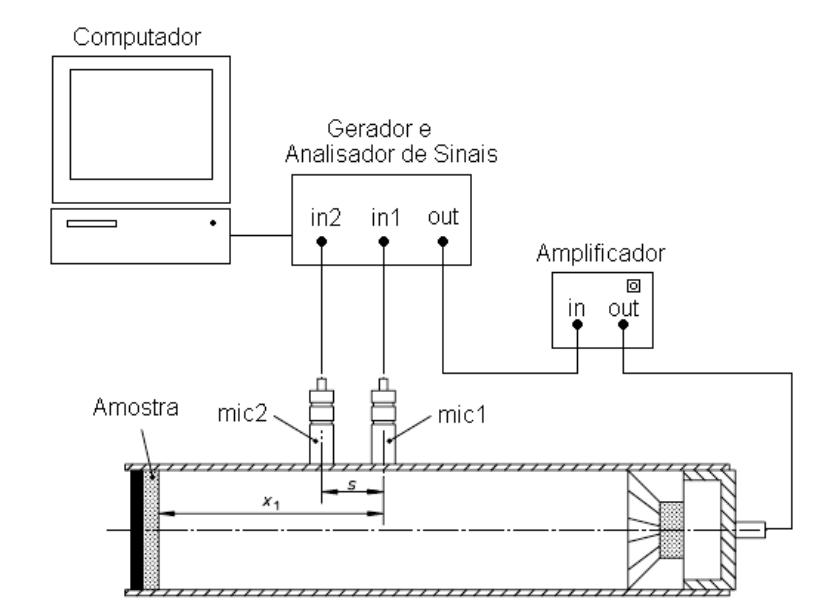
\includegraphics[scale=0.45]{figs/bancada.png}
\caption{Equipamentos utilizados para a medição a determinação do coeficiente de absorção sonora de um material em um tubo de impedância. Fonte \cite{mareze2013analise}}
\label{fig.equipamento}
\end{figure}  

\begin{table}[h]
\centering
\caption{Equipamentos utilizados na medição.}
\label{tab.bancada}
\begin{tabular}{l|l}
Item               & Descrição do Equipamento                                 \\ \hline
1                  & Analisador de sinais B\&K Pulse             \\
2                  & Computador com o programa Pulse LabShop       \\
3                  & Amplificador B\&K 2619\                    \\
4                  & Microfones de 1/2'' modelo B\&K 4189         \\
5                  & Calibrador 200 Larson Davids \\
                                                        
\end{tabular}
\end{table}

O material poroso analisado foi uma lã de vidro produzido pela empresa \textit{Rockfibras}, conforme a Figura \ref{fig.rockfibras}. Primeiramente foi feita a medição da função de transferência entre os microfones sem a presença do material poroso com o intuito de verificar se há absorção sonora nas superfícies do tubo, visto que as superfícies não são idealmente rígidas.
\begin{figure}[h]
\centering
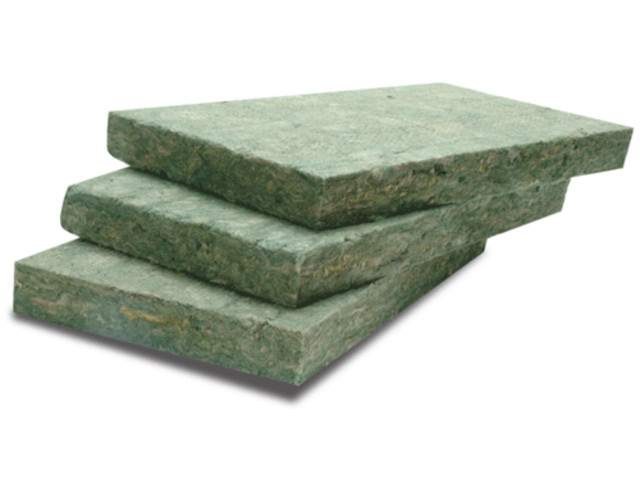
\includegraphics[scale=0.35]{figs/rockfibras.jpg}
\caption{Lã de rocha utilizada para o ensaio.}
\label{fig.rockfibras}
\end{figure}



Posteriormente foi recortada três (3) amostras de lã de vidro do mesmo material, porém com espessuras $h$ ligeiramente diferentes, exibidas na Tabela \ref{tab.espessuras}. O objetivo foi medir separadamente cada uma das amostras e verificar se o coeficiente de absorção sonora teve resultados semelhantes para os três ensaios.

\begin{table}[h]
\centering
\caption{Espessuras das amostras ensaiadas}
\label{tab.espessuras}
\begin{tabular}{l|l}
Item                       & Espessura (mm)      \\ \hline
Amostrador                 & 23.15               \\
Amostra 1                  & 25                  \\
Amostra 2                  & 24.85               \\
Amostra 3                  & 24                  \\
\end{tabular}
\end{table}

Para cada medição foi extraído como resposta as funções de transferências $H_{12}$ através de um \textit{template} programado no software Pulse LabShop. Como já foi discutido anteriormente, a partir das funções de transferência entre os microfones é possível extrair o coeficiente de absorção sonora por incidência direta de um material.

\chapter{Resultados}